\documentclass[12pt]{beamer} 
\usepackage{makecell}
\usepackage[utf8]{inputenc}
\usepackage[T1]{fontenc}
\usepackage[gen]{eurosym}
\usepackage{amsthm}
\usepackage{amsmath,amssymb,amsfonts}
\usepackage{graphicx}
\usepackage[authoryear]{natbib}
\usepackage{color}
\usepackage[polish]{babel}
\usepackage{hyperref}
\usepackage{url}

\usetheme{Berlin} 
\usecolortheme{seahorse}

\setbeamertemplate{theorems}[numbered]
\setbeamercolor{alerted text}{fg=red}
\setbeamercolor{block title exm}{bg=green!30!gray}

\theoremstyle{plain}

\newtheorem{thm}{Twierdzenie}
\newtheorem{defi}{Definicja}
\newtheorem{alg}{Algorytm}
\newtheorem{aten}{Uwaga}
\newtheorem{exm}{Przykład}

\begin{document}
\title{Systemy Liczbowe}
\subtitle{Technologie Informacyjne}
\author{Andrij Anrijczuk}
\date{Poznań 2025}
\institute{Politechnika Poznańska}

\begin{frame}
\titlepage
\vspace{-0,6cm}
\begin{figure}[h]
    \centering
    
\includegraphics[height=0.6in]{logopp.jpg}
    \end{figure}
\end{frame}

\begin{frame}
\tableofcontents
\end{frame}

\section{Wstęp}\label{sec:1}
\subsection{Troche o sobie}

\begin{frame}
\frametitle{Wstęp}
Na początku kilka  słów o sobie: \pause
\begin{itemize}
\item jestem z {\bf \textcolor{blue}{Ukra}}{\bf \textcolor{yellow}{iny}}  \pause
\item skończyłem {\bf \textcolor{cyan}{Liceum Nowojaworiwskie}}\pause
\item mam dużo hobby: \pause {\bf \textcolor{green}{pisarstwo}}\pause, {\bf \textcolor{green}{gotowanie}}\pause, {\bf \textcolor{green}{tworzenie gier}}\pause
\item studiuję się na Automatykę i Robotykę, dla tego, że chcę {\bf \textcolor{purple}{wcielić w życie dużo swoich idej}}
\end{itemize}
\end{frame}

\section{Pierwsze systemy liczb}
\subsection{Najstarszy system liczbowy}

\begin{frame}
\frametitle{Pierwsze systemy liczbowe}
\pause
\begin{thm}
Najstarszy wiadomy system liczbowy \pause - liczba na palcach
\end{thm} 
\begin{figure}
    \centering
    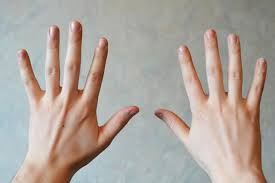
\includegraphics[width=0.5\linewidth]{Hands.jpg}
    \caption{Ręce \cite{ręce}}
    \label{fig:placeholder}
\end{figure}
\end{frame}

\subsection{Liczenie za pomocą nacięć}

\begin{frame}
\frametitle{Liczenie za pomocą nacięć}
\pause
\begin{defi}
Liczenie za pomocą nacięć - metoda liczenia, polegająca na rysowaniu pionowych kresek, grupowanych zazwyczaj po pięć, gdzie piąta kreska przekreśla cztery poprzednie
\end{defi} \pause
\begin{figure}
    \centering
    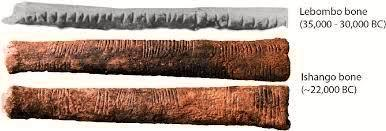
\includegraphics[width=0.8\linewidth]{Kości.jpg}
    \caption{Kości Lebombo i Iszango \cite{kości}}
    \label{fig:placeholder}
\end{figure}
\end{frame}

\section{Systemy dodawania liczb}
\subsection{Starożytny egipski system liczbowy}

\begin{frame}
\frametitle{Starożytny egipski system liczbowy}
\begin{table}
\begin{tabular}{| c | c | c | c |}
    \hline 
    \makecell{Liczba} & \makecell{Starożytny \\ hieroglif egipski} & \makecell{Liczba} & \makecell{Starożytny \\ hieroglif egipski} \\ 
    \hline 
    1 & $
\includegraphics[width=0.4cm]{Line_1.png}$ & 10000 & $
\includegraphics[width=0.25cm]{Finger_10000.png}$ \\ 
    \hline 
    10 & $
\includegraphics[width=0.4cm]{Loop_10.png}$ & 100000 & $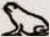
\includegraphics[width=0.8cm]{Frog_100000.png}$ \\ 
    \hline 
    100 & $
\includegraphics[width=0.6cm]{Spiral_100.png}$ & 1000000 & $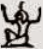
\includegraphics[width=0.8cm]{God_1000000.png}$ \\ 
    \hline 
    1000 & $
\includegraphics[width=0.4cm]{Lotos_1000.png}$ & & \\ 
    \hline 
\end{tabular}
\bigskip
\caption{Starożytny egipski system liczbowy \cite{egipski_znaki}}
\end{table}
\end{frame}

\begin{frame}
\frametitle{Starożytny egipski system liczbowy}
\begin{exm}
$$
\text{24 + 17 = 41}
$$
$$
\left( \cap \cap \text{ IIII} \right) + \left( \cap \text{ IIIIIII} \right) = \cap \cap \cap \text{ IIIIIIIIIII}
$$
$$
\implies \cap \cap \cap \underbrace{ \text{ IIIIIIIIII} }_{ = \cap } \text{ I}
$$
$$
\implies \cap \cap \cap \cap \text{ I} \quad 
$$
\end{exm}
\end{frame}

\subsection{Starożytny rymski system liczbowy}

\begin{frame}
\frametitle{Starożytny rymski system liczbowy}
\begin{table}
    
\begin{tabular}{| c | c | c | c |} 
    \hline 
    \makecell{Liczba} & \makecell{Starożytny \\ hieroglif rzymski} & \makecell{Liczba} & \makecell{Starożytny \\ hieroglif rzymski} \\ 
    \hline 
    1 & I & 100 & C \\ 
    \hline 
    5 & V & 500 & D \\ 
    \hline 
    10 & X & 1000 & M \\ 
    \hline 
    50 & L &  &  \\ 
    \hline 
\end{tabular}
\caption{Starożytny rymski system liczbowy}
\end{table}
\end{frame}

\begin{frame}
\frametitle{Starożytny rymski system liczbowy}
\begin{exm}
$$
\text{24 + 17 = 41}
$$
$$
\left( \text{XXIV} \right) + \left( \text{XVII} \right) = \text{XXXVVIIIII}
$$
$$
\implies \text{XXX} \cdot \underbrace{\text{VV}}_{\text{=X}} \cdot \text{III}
$$
$$
\implies \underbrace{\text{XXXXIII}}_{\text{XXXX} \rightarrow \text{XL}}
$$
$$
\implies \text{XLIII} \quad \text
$$
\end{exm}
\end{frame}

\section{Pozycyjne systemy liczby}

\begin{frame}
\frametitle{Pozycyjne systemy liczby}
\begin{defi}
    Systemy pozycyjne to metody zapisywania liczb, w których wartość cyfry zależy od jej miejsca (pozycji) w całym ciągu cyfr.
\end{defi}
\end{frame}

\subsection{Babiloński i sumeryjski system liczbowy}

\begin{frame}
\frametitle{Babiloński i sumeryjski system liczbowy}
\begin{itemize}
    \item \textbf{Wynalezienie pozycyjnego systemu liczbowego:} Wartość cyfry teraz zależy od jej pozycji.
    \item \textbf{Sześćdziesiętny system liczbowy:} Ten system był o wiele wygodniejszy do \textbf{obliczeń} oraz \textbf{mierzenia czasu}.
\end{itemize}
\end{frame}

\begin{frame}
\frametitle{Babiloński i sumeryjski system liczbowy}
\begin{thm} 
    Narody arabskie i indyjskie udoskonaliły ten system, dodając do niego \textbf{nic}, czyli \textbf{zero}.
\end{thm} \pause

\begin{equation}
    \sum_{n=0}^{\infty} \frac{f^{(n)}(a)}{n!} (x-a)^n \tag{Wzór Taylora}
\end{equation}
\end{frame}

\section{Binarny system liczby}

\begin{frame}
\frametitle{Binarny system liczby}
\begin{itemize}
\item Dwójkowy (binarny) system liczbowy operuje jedynie na dwóch cyfrach: 0 i 1. \pause
\item Wartość liczby jest określana przez pozycję każdej cyfry, lecz zamiast potęg liczby 10, wykorzystywane są potęgi liczby 2 ($\dots, 2^3, 2^2, 2^1, 2^0$).\pause
\begin{exm}
$$
\text{1010} \implies \text{$1 \cdot 2^3 + 0 \cdot 2^2 + 1 \cdot 2^1 + 0 \cdot 2^0$}
$$
$$
\implies \text{$8 + 0 + 2 + 0 = 10$}
$$
\end{exm}
\end{itemize}
\end{frame}

\begin{frame}
\frametitle{Binarny system liczby}
\begin{itemize}
\item System binarny jest bezpośrednio powiązany z Algebrą Boole’a (Boolean Algebra), gdzie 1 oznacza „Prawdę”, a 0 – „Fałsz”. \pause
\item Bity są grupowane w większe jednostki przechowywania danych:
\begin{itemize}
\item Bajt (Byte): 8 bitów.
\item Kilobajt (Kilobyte), Megabajt, Gigabajt: Wyższe jednostki, które są oparte na potęgach dwójki ($2^{10} = 1024$).
\end{itemize}
\end{itemize}
\end{frame}

\section{Podsumowanie}

\begin{frame}
\frametitle{Podsumowanie}
\centering
\vspace{0.5cm}
\begin{itemize}[<+->] % Elementy pojawiają się sekwencyjnie
    \item Zobaczyliśmy, jak \textbf{ewoluowały systemy liczbowe} — od palców do nowoczesnej logiki.
    \item Dowiedzieliśmy się o pochodzeniu \textbf{znanych nam system liczbowych}.
    \item Zrozumieliśmy zasadę działania \textbf{binarnego systemu liczbowego}, co daje nam lepsze rozumienie techniki i \textbf{zasady działania komputerów}.
\end{itemize}
\end{frame}

\section{Literatura}

\begin{frame}
\frametitle{Literatura}
\footnotesize % Зменшуємо розмір, щоб вмістити довгі посилання
\begin{thebibliography}{2}

\bibitem[Crilly(2009)]{RefTC}
Crilly, T. (2009). {\em 50 teorii matematyki, które każdy powinien znać}. PWN, Warszawa.

% ВИПРАВЛЕНО: Додано текст перед \url, щоб уникнути помилок форматування.
\bibitem{ręce} Źródło ilustracji (Ręce):
\url{https://www.rd.com/list/facts-you-learned-no-longer-true/} 
% Примітка: Довга URL-адреса була скорочена для кращого вигляду.

% ВИПРАВЛЕНО: Додано текст перед \url.
\bibitem{kości} Źródło ilustracji (Kości Lebombo i Iszango):
\url{https://theafricanhistory.com/341}
% Примітка: Довга URL-адреса була скорочена для кращого вигляду.

% ВИПРАВЛЕНО: Додано опис та видалено зайві символи з \url.
\bibitem{egipski_znaki} Grigorczuk, K. (2021). O systemach liczenia i mierzenia. \textit{Światopogląd}, 16(3), 11-18.
\url{https://www.mao.kiev.ua/biblio/jscans/svitogliad/svit-2021-16-3/svitoglyad-3-2021-grigorchuk-011.pdf}

\bibitem{RefO} Gemini, mój asystent SI
\url{https://gemini.google.com/app}

\end{thebibliography}
\end{frame}

\begin{frame}
    \vfill % Розміщує наступний елемент вертикально по центру
    
    \begin{center}
        \Huge\textbf{Dziękuję za uwagę} \\
        \vspace{1cm}
        \Large Macie jakieś pytania?
    \end{center}
    \vfill % Розміщує наступний елемент вертикально по центру
\end{frame}

\end{document}
